
\chapter{Heuristic algorithms}
\label{chap:Heuristic}

\start{C}{omputing} optimal solutions is intractable for many optimization problems of industrial and scientific importance. Unlike exact optimization algorithms, i.e., methods theoretically supported, heuristics do not guarantee the optimality of the obtained permutation, but they provide sub-optimal solutions. Moreover, they do not asses how close the obtained permutations are  from the optimal ones. In this chapter we will describe two type of methods: \textit{local search}  and \textit{greedy} algorithms. Local search algorithms are used by metaheuristic algorithms to improve the objective function, while greedy methods provide an initial permutation used by metaheuristic methods to start with. For each one we will report preliminary results. 

\paragraph{Notation} \mbox{}\\
 Since \textit{one-line} notation is used, often we will consider the permutation $\pi$ as a vector $\tilde{\bm \pi}$, where $\pi(i)=j$ becomes $\tilde{\pi}_i=j$. 



\section{Local search algorithms}
\label{sec:LocalSearch}
As the name suggests, local search algorithms seek a local optimum, i.e., an optimum in a neighborhood. 

\subsection{Preliminary definitions and results }


\noindent We present some theoretical definitions and result.

\begin{defi}[Distance between permutation]
	Let $\pi,\sigma \in \Sn$ be two permutations. Define the \textit{distance} between $\pi$ and $\sigma$ as the  numbers of indices at which the corresponding images are different, i.e.,
	\[
	\dist(\pi,\sigma):=\abs*{\{i: \pi(i)\neq \sigma(i)\}}.
	\]
\end{defi}
\noindent Sometimes this distance is called Hamming distance, from the American mathematician Richard Hamming.
\begin{oss}
	\label{rem:Distanza}
	This distance is also a topological distance. Moreover, we can observe that there are no permutations with distance $1$ between them.
\end{oss}

\begin{defi}[Neighborhood of radius $r$]\index{neighborhood of radius $r$}
	\label{def:Intorno}
	Let $\pi \in  S_n$ be a permutation and $r \ge 1$ be  an integer number.
Define the \textit{neighborhood} of center $\pi$ and radius $r$  as follows:
	\[
	N_{r}(\pi):=\{\sigma \in  S_n \mid \dist(\pi,\sigma)=r\}.
	\]	
\end{defi}
\begin{oss}
	From remark~\ref{rem:Distanza} it follows that $r$ cannot be $1$.
\end{oss}

\begin{defi}[Composition of permutations]
	Let $\pi,\sigma \in \Sn$. The permutation $\pi \cdot \sigma$ such that
	\[
	\left(\pi \cdot \sigma \right)(i) = \pi \left( \sigma (i) \right) \qquad \forall i=1,\dots,n
	\]
is called a \textit{composition} of $\pi$ and $\sigma$.
\end{defi}

\begin{defi}
Let $\pi \in \Sn$ be a permutation. The \textit{support} of $\pi$ is the set
\[
\supp{(\pi)} := \left\{i \mid i\in\{1,2,\dots,n\}, \, \pi(i) \neq i\right\}
\] 
of the elements \virgolette{moved} by $\pi$.
\end{defi}


\begin{defi}[$r$-exchange] \index{$r$-exchange}
Let $\pi,\sigma\in \Sn$ be two permutations and $r\in \N$ such that $2 \le r \le n$. If $\supp(\sigma) = r$, then $\pi \cdot \sigma$ is called a \textit{$r$-exchange} of $\pi$.
\end{defi}

%\begin{comment}
For example, let $\pi=[3,1,4,2]$, $\sigma =[2,1,3,4]$ and $\tau=[1,4,2,3]$.

First, note that $\abs{\supp(\sigma)}=\abs{\{1,2\}}=2$ and $\abs{\supp(\tau)}=\abs{\{2,3,4\}}=3$. 

Then, via composition we obtain that 
\begin{gather*}
\pi \cdot \sigma  = [\colorbox{green!30}{$3$},\colorbox{blue!20}{$1$},4,2]
 \cdot [\colorbox{gray!20}{$2$},\colorbox{gray!20}{$1$},3,4] =  [\colorbox{blue!20}{$1$},\colorbox{green!30}{$3$},4,2]\\
\intertext{is a $2$-exchange and}
\pi \cdot \tau = [3,\colorbox{orange!30}{$1$},\colorbox{cyan!30}{$4$},\colorbox{pink!30}{$2$}] \cdot [1,\colorbox{gray!20}{$4$},\colorbox{gray!20}{$2$},\colorbox{gray!20}{$3$}]= [3,\colorbox{pink!30}{$2$},\colorbox{orange!30}{$1$},\colorbox{cyan!30}{$4$}]
\end{gather*}
is a $3$-exchange.

Proposition~\ref{prop:Intorno} conveys the idea of the magnitude of a neighborhood $\insiemi N_r$ is. We did not find a proof of this in the literature, therefore we include it for sake of completeness
\begin{prop}
	\label{prop:Intorno}
	Let $\pi \in \Sn$ a permutation. It follows that 
	\begin{enumerate}
		\item The family of sets $\Big\{\{\pi\},\  N_{2}(\pi),\  N_{3}(\pi), \ \dots, \  N_{n}(\pi)\Big\}$ is a partition of $\Sn$;
		\item
		\(
		\displaystyle\abs{ N_r(\pi)}=\binom{n}{r}r!\sum_{i=2}^r \frac{(-1)^i}{i!}
		\) for every $\pi \in  S_n$.
	\end{enumerate}
\end{prop}
\begin{proof}
	The first statement follows from the definition of the neighborhood~$N_r$. 
	
	As regards the second point, let $\pi \in \Sn$ be a permutation.
	
	First, note that there are $\binom{n}{r}$ possible way to choose a subset of $r$ elements from a set of $n$ numbers. 
	
	Now, without loss of generality, we can consider $\pi = \mathrm{id}$, where $\mathrm{id}$ is the identity permutation, i.e., $\mathrm{id}(i)=i$ for every $i=1,\dots,n$.
	
	The number of possible permutation after a $r$-exchange with $\pi$ is equivalent to the numbers of permutation of $r$ elements with no fixed points (called derangements). 
	
	Therefore, for every $\pi \in \Sn$, $\abs{N_r (\pi)}  = \binom{n}{r} \, \cdot  \, !r$, where $!r$ is the number of derangement of a set of size $r$.
	
	It is well-known~\cite[(1)]{Weisstein} that the number of derangement of $r$ elements is
	\[
	!r = r! \cdot \sum_{i=0}^r \frac{(-1)^i}{i!}.
	\]
	
	\noindent Finally, the second statement follows, since $\sum_{i=0}^r \frac{(-1)^i}{i!}=\sum_{i=2}^r \frac{(-1)^i}{i!}$.
\end{proof}
\begin{cor}
	\label{cor:Intorni}
	From point 2, it follows that
	\begin{itemize}
		\item $\abs{ N_2(\pi)}=\binom{n}{2} = \frac{n^2-n}{2}$.
		\item  $\abs{ N_3(\pi)}=2\, \binom{n}{3} =  \frac{n^3-3n^2+2n}{3}$.
	\end{itemize} 
\end{cor}


Corollary~\ref{cor:Intorni} implies that doing a complete visit of $N_2$ requires $O(n^2)$ operations, while visiting $N_3$ requires $O(n^3)$ operations.

\begin{defi}
	A permutation $\pi^* \in S_n$ is called a \textit{$r$-optimum} (or \textit{$r$-~optimal}) if $z(\pi^*) \le z(\sigma)$ for every $\sigma \in N_r(\pi^*)$.
	An algorithm is called \textit{$r$-optimum} if it provides a $r$-optimal permutation.
\end{defi}


\subsubsection{Basics on $r$-optimum algorithms}

\noindent We are going to study two kinds of $r$-optimum algorithms:
\begin{enumerate}

	\item \textbf{First improvement:}  	this algorithm explores the $r$-neighborhood centered in the initial permutation and stops as soon as a reduction of the value of the objective function is obtained. Then, the exploration starts again from the $r$-neighborhood centered in the best permutation found. In the worst case (i.e., when no improvement is found), a complete evaluation	of the neighborhood is performed.
		\item \textbf{Best improvement:} this algorithm tries every $r$-exchange and chooses the best one. Hence, the exploration of the $r$-neighborhood is exhaustive, and all possible moves are examined to select the best neighboring permutation. This form of exploration may  result in a longer running time for large neighborhoods.
\end{enumerate}








\noindent For $r=4$ proposition~\eqref{prop:Intorno} tell us that visiting the whole neighbor has a computational cost of $O(n^4)$ operations. Thus, it is not worth to investigate cases for $r\ge 4$. Therefore, this thesis focuses on cases $r=2$ and $r=3$.



Every $r$-optimum algorithm has the same input and output:
\begin{description}
	\item[Input] The starting permutation $p$.
	\item[Output] 
	 The final permutation $m$ and its objective function value $z_m=z(m)$.
\end{description}



Finally, we will discuss briefly the notation used in the next pages.
\subsubsection{Notation}


For sake of clarity, in the following pages $\pi_{i_1 i_2}$ will denote the composition of $\pi \cdot \sigma$. 

For example, if $\pi=[3,1,4,2]$, then $\pi_{12}=[1,3,4,2]$. 

Sometimes we will refer to this $2$-exchange as $\{1,2\}\to \{2,1\}$.


	In table~\ref{tab:NomiAlgLocSearch} we report the algorithms we considered and the abbreviation we will use to refer to them.


\begin{table}
\caption{Name of local search algorithms}
\label{tab:NomiAlgLocSearch}	
	\centering
	\begin{tabular}{lcl}
	\toprule
	Name of the algorithm & $r$ & Abbreviation \\
	\midrule
	$2$-optimum first improvement & $2$ & \texttt{2optFirst} \\
		$2$-optimum best improvement & $2$ & \texttt{2optBest} \\
			$3$-optimum first improvement & $3$ & \texttt{3optFirst} \\
				$3$-optimum best improvement & $3$ & \texttt{3optBest} \\
	\bottomrule	
	\end{tabular}
\end{table}


\subsection{Preliminary on $2$-optimum algorithms}
The first $2$-optimum algorithm for QAP was studied by Charles H. Heider in 1973~\cite{Heider1973}. 



In order to reduce the overall computational cost associated to evaluation of the objective function $z$, it is possible to proceed as follows.



Let $\pi \in \Sn$ and fix two indices $i_1 \neq i_2$ of $[n]$. In the following results let $\pi_{i_1 i_2}$ denote the permutation obtained by $\pi$, exchanging the indices $i_1$ and $i_2$, i.e.,

\[
\pi_{i_1 i_2}(i) :=
\begin{cases}
\pi(i_2) & \text{if $i = i_1$;} \\
\pi(i_1) & \text{if $i = i_2$;} \\
\pi(i)   & \text{otherwise.} \\
\end{cases}
\]

\begin{defi}\label{def:Delta}
	Let $\pi \in \Sn$  and fix two indices $i_1 \neq i_2 \in \In$. 
	Let  $\Delta(\pi; i_1,i_2)$ be defined  as
	\begin{equation}\label{eq:defDelta}
	\begin{split}
	\Delta(\pi;i_1,i_2):&=\left(f_{i_1i_1}-f_{i_2i_2}\right)\left(d_{\pi(i_2)\pi(i_2)}-d_{\pi(i_1)\pi(i_1)}\right)\\
	&+\left(f_{i_1i_2}-f_{i_2i_1}\right)\left(d_{\pi(i_2)\pi(i_1)}-d_{\pi(i_1)\pi(i_2)}\right) \\
	&+\sum_{j \notin\left\{i_1,i_2\right\}} \Big\{\left(f_{i_1j}-f_{i_2j}\right)\left(d_{\pi(i_2)\pi(j)}-d_{\pi(i_1)\pi(j)}\right)\\
	&\phantom{\sum_{j \notin\left\{i_1,i_2\right\}}+}+\left(f_{j i_1}-f_{ji_2}\right)\left(d_{\pi(j)\pi(i_2)}-d_{\pi(j)\pi(i_1)}\right)\Big\}. 
	\end{split}
	\end{equation}
\end{defi}



\begin{oss}
	If the matrices $\bm F$ and $\bm D$ are symmetric, then the formula~\eqref{eq:defDelta} becomes
	\begin{equation}
	\Delta(\pi; i_1,i_2) = 2 \sum_{j \notin\left\{i_1,i_2\right\}}\left(f_{j i_1}-f_{ji_2}\right)\left(d_{\pi(j)\pi(i_2)}-d_{\pi(j)\pi(i_1)}\right).
	\end{equation}
\end{oss}
\begin{oss}
	The evaluation of $\Delta(\pi; i_1,i_2)$ requires $2(n-2)+2=2n-2$ products and $6n-7$ sums. In the symmetric case, the evaluation requires $n-1$ products and $3n-6$ sums. In every case, $\Delta$ can be evaluated in $O(n)$ operations.
\end{oss}

\begin{teo}
	\label{teo:2optDelta}
	Let $\pi \in \Sn$ be a permutation and $i_1 \neq i_2$ be  two indices. Then, 
	\begin{equation}
	z(\pi_{i_1 i_2}) = z(\pi) + \Delta(\pi; i_1,i_2).
	\end{equation} 
\end{teo}
We did not find a proof of this in the literature, therefore we include it in Appendix~\ref{AppendiceA} for the sake of completeness. 


Observe that theorem~\ref{teo:2optDelta} allows us to evaluate the difference between a permutation $\pi$ and its $2$-exchange $\pi_{i_1i_2}$ with a cost of $O(n)$ operations. 

Taking account that the straightforward evaluation of a quadratic objective function has a cost of $O(n^2)$, we got the conclusion that the approach described below, exploiting the structure of the problem, allows us to save some computational time.


\subsection{$2$-optimum: First improvement}

\subsubsection{Description of the algorithm}


\noindent A detailed description of this algorithm can be found in pseudo code~\ref{Pseudocode:2optFirst}.

\begin{algorithm}

	\KwIn{$n$,$\bm F$,$\bm D$, $p$}
	\KwOut{$m$, $z_m$}
	\tcc{initialization}
	Evaluate $z_p = z(p)$\;
	$m \gets p$\; 
	$z_m \gets z_p$\;
	\tcc{main loop}
	\For{$i_1 =1,\dots, n-1 $}{
		\label{alg:primeramejora}
		\For{$i_2=i_1+1,\dots, n$}{
			Evaluate $\Delta(m;i_1,i_2)$\;
			\If{$\Delta(m;i_1,i_2)< 0$ }{
				$z_m \gets z_m + \Delta(m;i_1,i_2)$\;
				Do the $2$-exchange $m \gets m_{i_1i_2}$\;
				Go to step~\ref{alg:primeramejora}\;
			}		
		}
	}
	
	Stop: $m$ is  $2$-optimal with value $z_m$.	
	\caption{$2$-optimum, first improvement}
	\label{Pseudocode:2optFirst}
\end{algorithm}

We can see that there are two \texttt{DO} cycles (lines 4-5), in order to try every $2$-exchange of the current permutation $m$.

In every step, the algorithm evaluates the term $\Delta$ until it finds a $2$-exchange which improves the current permutation (lines 6 - 11).
This is achieved by the \texttt{IF} cycle in line 7: if $\Delta(m,i_1,i_2)<0$, then the $2$ exchange $m_{i_1i_2}$ has a lower objective function value than $m$.

Then, the algorithm performs the $2$-exchange and starts again from $m_{i_1i_2}$ (lines 9-10).

The algorithm stops whenever there are no $2$-exchange that improve the current permutation, i.e., when $\Delta(m,i_1,i_2)\ge 0$ for every $i_1,i_2\in\{1,\dots,n\}$.

Hence, the final permutation is $2$-optimum because there are no more $2$-exchange available and every $2$-exchange increase the objective function value.

Note that this is a finite termination algorithm because there are a finite number of permutations. Thus, the algorithm performs a finite numbers of iterations.

\subsubsection{Complexity of the algorithm}
%\noindent 
In the best case, an incrementing $2$-exchange is always found in the first attempt, so in lines 5 - 12 the algorithm requires only one $\Delta$-evaluation.

The cost of evaluating  $\Delta$ is $O(n)$ operations.

 Hence, the final cost of lines 4 - 13 in the best case is $O(n)$ operations.

In the worst case, the incrementing $2$-exchange is found at the end of the loops in steps 4-5.
Since the algorithm tests every possible $2$-exchange, the number of evaluations done in lines 4 - 13 is 
\begin{equation}
\label{eq:NumValut2Ottimi}
\begin{split}
\sum_{i_1=1}^{n-1}\sum_{i_2=i_1+1}^n 1 &= \sum_{i_1=1}^{n-1} (n-i_1) \\
&=  \sum_{i_1=1}^{n-1} n - \sum_{i_1=1}^{n-1}i_1 \\
&= n \cdot (n-1) - \frac{n}{2}\cdot (n-1) \\
&= \frac{n(n-1)}{2} = \binom{n}{2},
\end{split}
\end{equation}
\noindent as a further evidence of the proposition~\ref{prop:Intorno}. 

Since the evaluation cost of $\Delta$ is $O(n)$ operations, the total cost of lines 4-13 in worst case is $O(n^3)$.

These costs are repeated for every $2$-exchange made. There are no way to evaluate \textit{a priori} how many $2$-exchanges the algorithm is gonna do, but we are going to try some tests in Section~\ref{sec:r-ottimi}.




\subsubsection{An example}

\noindent A basic example is described in table~\ref{tab:esempio2optfirst}. Instance \texttt{Neos4} was used. See Section~\ref{sec:NEOS} for more details.

The quality of a permutation is defined by the  Percent Deviation (PD) from the best known solution, calculated according to 
\begin{equation}\label{eq:PD}
	\operatorname{PD}(z,z_\mathrm{BKS}):=\frac{z-z_\mathrm{BKS}}{z_\mathrm{BKS}}\cdot 100,
\end{equation}
\noindent where $z$  is the obtained permutation and $z_\mathrm{BKS}$ is the best known solution (or the optimum) of the corresponding problem.

\begin{table}%[htp]
	\footnotesize
	\centering
\caption{Example of \texttt{2optfirst} algorithm}
\label{tab:esempio2optfirst}
	\begin{tabular}{*{6}{S[table-format =1.0]}S[table-format =3.0]l}
		\toprule
\multicolumn{2}{c}{{Indices}}& \multicolumn{4}{c}{{Permutation}} &{Cost}& Remarks \\		
\cmidrule(lr){1-2}
\cmidrule(lr){3-6}
		 {$i_1$}& {$i_2$}& 1 & 2 & 3 & 4 &  & \\		
		\midrule
& & 1 &2 &3 &4 &  908 &Initial permutation\\
1 &2 && & & &  926 &No improvement\\
1 &3 && & & & 1008 &No improvement\\
1 &4 && & & & 1052 &No improvement\\
2 &3 && & & & 1136 &No improvement\\
2&4 &  & & & &  850 &Exchange locations 2 and 4\\
& & 1 &4 &3 &2 &  850 &Start again\\
1 &2 && & & &  930 &No improvement\\
1&3 &  & & & &  790 &Exchange locations 1 and 3\\
& & 3 &4 &1 &2 &  790 &Start again\\
1 &2 && & & &  834 &No improvement\\
1 &3 && & & &  850 &No improvement\\
1 &4 && & & & 1066 &No improvement\\
2 &3 && & & & 1018 &No improvement\\
2 &4 && & & & 1008 &No improvement\\
3 &4 && & & &  824 &No improvement\\
\midrule
& & 3 &4 &1 &2 &  790 &Best permutation found\\
\bottomrule
	\end{tabular}

\end{table}


In this case, the $2$-optimal permutation achieved is an optimum. This is, in general, not true.
In figure~\ref{fig:2optfirst} we plotted the objective function values versus the iterations. As we can see, as soon as the algorithm finds a permutation reducing the cost value, it starts again from this permutation, exploring its $r$-neighborhood.

\begin{figure}
	\centering
	\includegraphics[width=.75\textwidth]{2optFirst}
	\caption{\texttt{2optFirst} algorithm,  Objective function values versus the iterations.}
	\label{fig:2optfirst}
\end{figure}







\subsection{$2$-optimum: Best improvement}
\subsubsection{Description of the algorithm}
A detailed description of this algorithm can be found in pseudo code~\ref{Pseudocode: 2optBestImpr}.
\begin{algorithm}%[htp]
	\KwIn{$n$,$\bm F$,$\bm D$,$p$}
	\KwOut{$m$, $z_m$}
	\tcc{initialization}
	Evaluate $z_p =z(p)$\;
	$m\gets p$\; 
	$z_m \gets z_p$\;
	$d_\mathrm{min} \gets 0$\;\label{step:2optbest}
	\tcc{main loop}
	\For{$i_1 =1,\dots, n-1 $} 
	{
		\For{$i_2=i_1+1,\dots, n$}{
			Evaluate $\Delta(m;i_1,i_2)$\;
			\If{$\Delta(m;i_1,i_2)< d_\mathrm{min}$ }{
				$j_1 \gets i_1$\;
				$j_2 \gets i_2$\;
				$d_\mathrm{min} \gets \Delta(m;j_1,j_2)$\;
			}
		}
	}

	\If(\tcc*[f]{If $m$ is the new best permutation found}){$ d_\mathrm{min} < 0$}{
		$z_m \gets z_m + d_\mathrm{min}$\;
		Do the $2$-exchange $m \gets m_{i_1i_2}$\;
		Go to step~\ref{step:2optbest}\;			
	}
	
	\lIf{$d_\mathrm{min}=0$}{stop: $m$ is  $2$-optimal with value $z_m$}
	
	\caption{$2$-optimum: best improvement}
	\label{Pseudocode: 2optBestImpr}
\end{algorithm}



The \textit{best improvement} algorithm starts from a permutation $p$ with objective function value $z(p)=z_p$; it sets $m = p$, $z_m=z_p$ and  initializes $d_\mathrm{min}$ at $0$ (lines 1-4).

There are two  \texttt{DO} cycles, in order to try every possible  $2$-exchange of $p$ (lines 5 - 6).


For every $i_1$ and $i_2$, algorithm evaluates the term $\Delta(m;i_1,i_2)$ (line 7) and it computes the following term (lines 8-12):
\[ d_\mathrm{min}:=\min\Bigl\{\Delta(m;i_1,i_2) \, \big| \, i_1\in\{1,\dots,n-1\},i_2\in\{i_1+1,\dots,n\}\Bigr\}.\] 	 



\noindent Now, if $d_\mathrm{min}<0$, then the $2$-exchange is applied and $m$ and $z_m$ are updated (lines 15 - 17).

 The algorithm starts again from the new $m$ (line 18).

This procedure is repeated until $d_\mathrm{min}=0$ (note that $d_\mathrm{min}$ cannot be positive, since it is initialized as $0$).

Observe that since there are a finite numbers of permutations, the algorithm ends in a finite number of iterations.

In case $d_\mathrm{min}=0$, every possible $2$-exchange does not improve the objective function. Therefore, $m$ is $2$-optimal with objective function $z_m$ (line 20).

\subsubsection{Complexity of the algorithm}
Note that \texttt{2optBest} algorithm corresponds to the worst case of  \texttt{2optFirst}. Hence its computational cost is $O(n^3)$, as shown in equation~\eqref{eq:NumValut2Ottimi}.

\subsubsection{An example}
A basic example is described in table~\ref{tab:esempio2optbest}. Instance \texttt{Neos4} was used. See section~\ref{sec:NEOS} for more details.


\begin{table}%[htp]
	\footnotesize
	\centering
		\caption{Example of best improvement algorithm}
	\label{tab:esempio2optbest}
	\begin{tabular}{*{6}{S[table-format =1.0]}S[table-format =3.0]l}
	\toprule
	\multicolumn{2}{c}{{Indices}}& \multicolumn{4}{c}{{Permutation}} &{Cost}& Remarks \\		
	\cmidrule(lr){1-2}
	\cmidrule(lr){3-6}
	{$i_1$}& {$i_2$}& 1 & 2 & 3 & 4 &  & \\		
	\midrule
& & 1 &2 &3 &4 &  908 &Initial permutation\\
1 &2 && & & &  926 &No improvement\\
1 &3 && & & & 1008 &No improvement\\
1 &4 && & & & 1052 &No improvement\\
2 &3 && & & & 1136 &No improvement\\
2 &4 && & & &  850 &Improvement: store indices\\
3 &4 && & & &  864 &Improvement, but worst than 850\\
& & 1 &2 &3 &4 &  864 &Exchange locations $2$ and $4$\\
& & 1 &4 &3 &2 &  850 &Start again\\
1 &2 && & & &  930 &No improvement\\
1 &3 && & & &  790 &Improvement: store indices\\
1 &4 && & & &  990 &No improvement\\
2 &3 && & & &  982 &No improvement\\
2 &4 && & & &  908 &No improvement\\
3 &4 && & & &  960 &No improvement\\
& & 1 &4 &3 &2 &  960 &Exchange locations $1$ and $3$\\
& & 3 &4 &1 &2 &  790 &Start again\\
1 &2 && & & &  834 &No improvement\\
1 &3 && & & &  850 &No improvement\\
1 &4 && & & & 1066 &No improvement\\
2 &3 && & & & 1018 &No improvement\\
2 &4 && & & & 1008 &No improvement\\
3 &4 && & & &  824 &No improvement\\
\midrule
& & 3 &4 &1 &2 &  790 &Best permutation found\\
		\bottomrule
	\end{tabular}

\end{table}


%\bel{
	Note the main differences between Tables~\ref{tab:esempio2optbest} and~\ref{tab:esempio2optfirst}: when \texttt{2optBest} find an improvement of the objective function, it stores the indices of the improving $2$-exchange.  %}

As we can see, the algorithm achieves the optimal solution.
Figure~\ref{fig:2optbest} shows the variation of objective function value. We can clearly see that every cycle is repeated three times.

\begin{figure}
	\centering
	\includegraphics[width=.75\textwidth]{2optBest}
	\caption{\texttt{2optBest} algorithm, Objective function values  versus iterations.}
	\label{fig:2optbest}
\end{figure}






\subsection{Preliminary on $3$-optimum algorithms}
\label{sec:Preliminary3Opt}

The  $3$-optimum  algorithm  was  first   proposed   by   G. A. Croes~\cite{Croes1958}  in 1958    for   Travelling   Salesman   Problem.

These $3$-optimum algorithm are similar to the $2$-optimum algorithms except that they consider swapping three facilities at a time.

With three distinct indices $i_1$,$i_2$,$i_3$, one can obtain two kind of $3$-exchanges:
\begin{enumerate}
	\item $\{i_1,i_2,i_3\}\to\{i_2,i_3,i_1\}$.
	\item $\{i_1,i_2,i_3\}\to\{i_3,i_1,i_2\}$.
\end{enumerate}
If $\pi \in \Sn$ is a permutation and $i_1$,$i_2$,$i_3 \in [n]$ are three distinct indices, define $\pi^1_{i_1i_2i_3} \in  N_3(\pi)$ as the permutation such that
\begin{equation}
\label{eq:pi^1}
\pi^1_{i_1i_2i_3}(j):=
\begin{cases}
\pi(i_2) & \text{if $j = i_1$;}\\
\pi(i_3) & \text{if $j = i_2$;}\\
\pi(i_1) & \text{if $j = i_3$;}\\
\pi(j)   & \text{otherwise.}
\end{cases}
\end{equation}
and $\pi^2_{i_1i_2i_3} \in  N_3(\pi)$ as 
\begin{equation}
\label{eq:pi^2}
\pi^2_{i_1i_2i_3}(j):=
\begin{cases}
\pi(i_3) & \text{if $j = i_1$;}\\
\pi(i_1) & \text{if $j = i_2$;}\\
\pi(i_2) & \text{if $j = i_3$;}\\
\pi(j)   & \text{otherwise.}
\end{cases}
\end{equation}

For example, if $\pi = [3,1,4,2]$, then
\[
\pi^2_{123}=[1,3,4.2]\qquad \text{and }
\pi^1_{123}=[4,3,1,2]\qquad .
\]
\begin{defi}
Let $\pi \in \Sn$ be a permutation and $i_1$,$i_2$,$i_3 \in [n]$ three distinct indices. 
Define $\varDelta^1(\pi;i_1,i_2,i_3)$ and $\varDelta^2(\pi;i_1,i_2,i_3)$ as follows.
\footnotesize
\begin{equation}
\label{eq:Delta1}
\begin{split}
\Delta^1(\pi;i_1,i_2,i_3)&:=
f_{i_1i_1}\left(d_{\pi(i_2)\pi(i_2)}-d_{\pi(i_1)\pi(i_1)}\right)
+f_{i_1i_2}\left(d_{\pi(i_2)\pi(i_3)}-d_{\pi(i_1)\pi(i_2)}\right)\\
&+f_{i_1i_3}\left(d_{\pi(i_2)\pi(i_1)}-d_{\pi(i_1)\pi(i_3)}\right)
+f_{i_2i_1}\left(d_{\pi(i_3)\pi(i_2)}-d_{\pi(i_2)\pi(i_1)}\right) \\
&+f_{i_2i_2}\left(d_{\pi(i_3)\pi(i_3)}-d_{\pi(i_2)\pi(i_2)}\right)
+f_{i_2i_3}\left(d_{\pi(i_3)\pi(i_1)}-d_{\pi(i_2)\pi(i_3)}\right) \\
&+f_{i_3i_1}\left(d_{\pi(i_1)\pi(i_2)}-d_{\pi(i_3)\pi(i_1)}\right)
+f_{i_3i_2}\left(d_{\pi(i_1)\pi(i_3)}-d_{\pi(i_3)\pi(i_2)}\right) \\
&+f_{i_3i_3}\left(d_{\pi(i_1)\pi(i_1)}-d_{\pi(i_3)\pi(i_3)}\right)\\
&+\sum_{j\notin\{i_1,i_2,i_3\}}\Big[
f_{i_1j}\left(d_{\pi(i_2)\pi(j)}-d_{\pi(i_1)\pi(j)}\right)
+f_{i_2j}\left(d_{\pi(i_3)\pi(j)}-d_{\pi(i_2)\pi(j)}\right)\\
&\qquad \qquad
+f_{i_3j}\left(d_{\pi(i_1)\pi(j)}-d_{\pi(i_3)\pi(j)}\right)
+f_{ji_1}\left(d_{\pi(j)\pi(i_2)}-d_{\pi(j)\pi(i_1)}\right) \\
&\qquad \qquad
+f_{ji_2}\left(d_{\pi(j)\pi(i_3)}-d_{\pi(j)\pi(i_2)}\right)
+f_{ji_3}\left(d_{\pi(j)\pi(i_1)}-d_{\pi(j)\pi(i_3)}\right) \Big].
\end{split}
\end{equation}	
\normalsize
and
\footnotesize
\begin{equation}
\label{eq:Delta2}
\begin{split}
\Delta^2(\pi;i_1,i_2,i_3)&:=
f_{i_1i_1}\left(d_{\pi(i_3)\pi(i_3)}-d_{\pi(i_1)\pi(i_1)}\right)
+f_{i_1i_2}\left(d_{\pi(i_3)\pi(i_1)}-d_{\pi(i_1)\pi(i_2)}\right)\\
&+f_{i_1i_3}\left(d_{\pi(i_3)\pi(i_2)}-d_{\pi(i_1)\pi(i_3)}\right)
+f_{i_2i_1}\left(d_{\pi(i_1)\pi(i_3)}-d_{\pi(i_2)\pi(i_1)}\right) \\
&+f_{i_2i_2}\left(d_{\pi(i_1)\pi(i_1)}-d_{\pi(i_2)\pi(i_2)}\right)
+f_{i_2i_3}\left(d_{\pi(i_1)\pi(i_2)}-d_{\pi(i_2)\pi(i_3)}\right) \\
&+f_{i_3i_1}\left(d_{\pi(i_2)\pi(i_3)}-d_{\pi(i_3)\pi(i_1)}\right)
+f_{i_3i_2}\left(d_{\pi(i_2)\pi(i_1)}-d_{\pi(i_3)\pi(i_2)}\right) \\
&+f_{i_3i_3}\left(d_{\pi(i_2)\pi(i_2)}-d_{\pi(i_3)\pi(i_3)}\right)\\
&+\sum_{j\notin\{i_1,i_2,i_3\}}\Big[
f_{i_1j}\left(d_{\pi(i_3)\pi(j)}-d_{\pi(i_1)\pi(j)}\right)
+f_{i_2j}\left(d_{\pi(i_1)\pi(j)}-d_{\pi(i_2)\pi(j)}\right)\\
&\qquad \qquad
+f_{i_3j}\left(d_{\pi(i_2)\pi(j)}-d_{\pi(i_3)\pi(j)}\right)
+f_{ji_1}\left(d_{\pi(j)\pi(i_3)}-d_{\pi(j)\pi(i_1)}\right) \\
&\qquad \qquad
+f_{ji_2}\left(d_{\pi(j)\pi(i_1)}-d_{\pi(j)\pi(i_2)}\right)
+f_{ji_3}\left(d_{\pi(j)\pi(i_2)}-d_{\pi(j)\pi(i_3)}\right) \Big].
\end{split}
\end{equation}	
\normalsize
\end{defi}

\begin{oss}
In symmetric \QAP($\bm F$,$\bm D$), equations~\eqref{eq:Delta1} and~\eqref{eq:Delta2} reduce to 
\footnotesize
\[
\begin{split}
\Delta^1(\pi;i_1,i_2,i_3)&:=
2\Big\{f_{i_1i_2}\left(d_{\pi(i_2)\pi(i_3)}-d_{\pi(i_1)\pi(i_2)}\right)
+f_{i_1i_3}\left(d_{\pi(i_2)\pi(i_1)}-d_{\pi(i_1)\pi(i_3)}\right)\\
&\quad
+f_{i_2i_3}\left(d_{\pi(i_1)\pi(i_3)}-d_{\pi(i_2)\pi(i_3)}\right) 
+f_{i_3i_3}\left(d_{\pi(i_1)\pi(i_1)}-d_{\pi(i_3)\pi(i_3)}\right)\\
&+\sum_{j\notin\{i_1,i_2,i_3\}}\Big[
f_{ji_1}\left(d_{\pi(j)\pi(i_2)}-d_{\pi(j)\pi(i_1)}\right)
+f_{ji_2}\left(d_{\pi(j)\pi(i_3)}-d_{\pi(j)\pi(i_2)}\right)\\
&\qquad \qquad \quad
+f_{ji_3}\left(d_{\pi(j)\pi(i_1)}-d_{\pi(j)\pi(i_3)}\right)
 \Big]
\Big\}
\end{split}
\]
\normalsize
and
\footnotesize
\[
\begin{split}
\Delta^2(\pi;i_1,i_2,i_3)&:=
2\Big\{f_{i_1i_2}\left(d_{\pi(i_1)\pi(i_3)}-d_{\pi(i_1)\pi(i_2)}\right)
+f_{i_1i_3}\left(d_{\pi(i_2)\pi(i_3)}-d_{\pi(i_1)\pi(i_3)}\right)\\
&\quad
+f_{i_2i_3}\left(d_{\pi(i_1)\pi(i_2)}-d_{\pi(i_2)\pi(i_3)}\right) 
+f_{i_3i_3}\left(d_{\pi(i_1)\pi(i_1)}-d_{\pi(i_3)\pi(i_3)}\right)\\
&+\sum_{j\notin\{i_1,i_2,i_3\}}\Big[
f_{ji_1}\left(d_{\pi(j)\pi(i_3)}-d_{\pi(j)\pi(i_1)}\right)
+f_{ji_2}\left(d_{\pi(j)\pi(i_1)}-d_{\pi(j)\pi(i_2)}\right)\\
&\qquad \qquad \quad
+f_{ji_3}\left(d_{\pi(j)\pi(i_2)}-d_{\pi(j)\pi(i_3)}\right)
\Big].
\Big\}
\end{split}
\]
\normalsize
\end{oss}

\begin{oss}
	%\bel{
		The evaluation of $\Delta^1$ and $\Delta^2$ requires $6n-9$ products and $12n-8$ sums. Respectively, in symmetric case, the evaluation of them requires $3n-5$ products and $6n-12$ sums.
	
	In every case, they can be evaluated in $O(n)$ operations.
\end{oss}

\begin{teo}
	\label{teo:3optDelta}
Let $\pi \in \Sn$ be a permutation and $i_1,i_2,i_3 \in [n]$ three distinct indices.  Then one has
\begin{itemize}
	\item $z\left(\pi^1_{i_1i_2i_3}\right)= z(\pi) +\Delta^1(\pi;i_1,i_2,i_3)$ 
	\item $z\left(\pi^2_{i_1i_2i_3}\right)= z(\pi) +\Delta^2(\pi;i_1,i_2,i_3)$ 
\end{itemize}
\end{teo}

We did not find a proof of this in the literature, therefore we include it here for the sake of completeness. The proof can be found on Appendix~\ref{AppendiceB}.

\newpage
\subsection{$3$-optimum: first improvement}

\subsubsection{Description of the algorithm}
A detailed description of this algorithm can be found in pseudo code~\ref{Pseudocode: 3optFirstImpr}.

\begin{algorithm}[htp]
	\KwIn{$n$,$\bm F$,$\bm D$,$p$}
	\KwOut{$m$, $z_m$}
	\tcc{initialisation}
	Read $p$\;
	Evaluate $z_p \gets z(p)$\;
	$z_m \gets z_p$ \;
	\tcc{main loops}
	\For{$i_1 =1,\dots, n-2 $} 
	{\label{step:3optbest}
		\For{$i_2=i_1+1,\dots, n-1$}{
			\For{$i_3=i_2+1,\dots,n $}{
				Evaluate $\Delta^1(m;i_1,i_2,i_3)$\;
				\If{$\Delta^1(m;i_1,i_2,i_3)< 0$ }{
					Do the $3$-exchange $m\gets m_{i_1i_2i_3}$\;
					$z_m \gets z_m + \Delta^1(m;i_1,i_2,i_3)$\;
					Goto step~\ref{step:3optbest}\;
				}
				Evaluate $\Delta^2(m;i_1,i_2,i_3)$\;	
				\If{$\Delta^2(m;i_1,i_2,i_3)<0$}{
					Do the $3$-exchange $m\gets m_{i_1i_2i_3}$\;
					$z_m \gets z_m + \Delta^2(m;i_1,i_2,i_3)$\;
					Goto step~\ref{step:3optbest}\;
				}
				
			}
		}
	}
	Stop: $m$ is  $3$-optimal with objective function value $z_m$.
	\caption{$3$-optimum: first improvement}
	\label{Pseudocode: 3optFirstImpr}
\end{algorithm}






This algorithm is fairly similar to \texttt{2optFist}. In fact, the algorithm updates that permutation as soon as it founds an improvement obtained by a $3$-exchange.

The main difference is that there are two possible $3$-exchanges that can be done. Thus, the algorithm evaluates both $\Delta^1$ and $\Delta^2$ terms.

\subsubsection{Complexity of the algorithm}
In the best case, the algorithm immediately finds an improving $3$-exchange with $\Delta^1<0$. Hence in this case, for every $3$-exchange, the computational cost of \texttt{3optFirst} is $O(n)$ operations.

In the worst case, the algorithm will find the improving $3$-exchange only at the end of each iterations. 
%\bel{
Equation~\eqref{eq:Calcoli3optFirst} shows us that \texttt{3optFirst}, in the worst case,  requires $\binom{n}{3}=O(n^3)$ loops, therefore the total cost in the worst case is $O(n^4)$ operations.
%}

\begin{equation}
\label{eq:Calcoli3optFirst}
\begin{split}
\sum_{i_1=1}^{n-2}\left(\sum_{i_2=i_1+1}^{n-1}\left(\sum_{i_3=i_2+1}^n 1\right)\right) 
&= \sum_{i_1=1}^{n-2}\left(\sum_{i_2=i_1+1}^{n-1} \left(n-i_2\right)\right) \\
&=\sum_{i_1=1}^{n-2}\frac{(n-i_1)(n-i_1-1)}{2}\\
&=\sum_{i_1=1}^{n-2}\binom{n-i_1}{2}\\
&=\sum_{j=2}^{n-1}\binom{j}{2}=\sum_{j=0}^{n-1}\binom{j}{2}=\binom{n}{3},
\end{split}
\end{equation}

\noindent where we used the known identity \[\sum_{j=0}^n\binom{j}{m}=\binom{n+1}{m+1}\]
(see (5.10) in Concrete Mathematicsby D. E. Knuth, O. Patashnik, and R. Graham).

\subsubsection{An example}

\noindent A basic example is described in table~\ref{tab:esempio3optfirst}, where \texttt{3optFirst} starts with initial permutation $[1,2,3,4,5]$. Instance \texttt{Neos5} was used; see section~\ref{sec:NEOS} for more details.


\begin{table}%[htp]
	\footnotesize
	\caption{Example of \texttt{3optFirst}.}
	\label{tab:esempio3optfirst}
	\centering
	\begin{tabular}{*{8}{S[table-format =1.0]}S[table-format =3.0]l}
		\toprule
		\multicolumn{3}{c}{{Indices}} &\multicolumn{5}{c}{{Permutation}} &{Cost}& Remarks \\		
		\cmidrule(lr){1-3}
		\cmidrule(lr){4-8}
		{$i_1$}& {$i_2$}& {$i_4$}	 & 1 & 2 & 3 & 4 & 5 & & \\		
		\midrule
		& & &1 &2 &3 &4 &5 &  900 &Initial permutation\\
1		&2 &3 & & & & & &  836 &Exchange locations 1, 2 and 3 with $\pi^1$\\
		& & &2 &3 &1 &4 &5 &  836 &Start again\\
	1	&2 &3 & & & & & &  780 &Exchange locations 1, 2 and 3 with $\pi^1$\\
		& & &3 &1 &2 &4 &5 &  780 &Start again\\
		1 & 2 & 3 & & & & & &  780 &No improvement\\
		1 & 2 & 4 & & & & & &  780 &No improvement\\
		1 & 2 & 5 & & & & & &  780 &No improvement\\
	1	& 3&4 & & & & & &  744 &Exchange locations 1, 3 and 4 with $\pi^1$\\
		& & &2 &1 &4 &3 &5 &  744 &Start again\\
	1	& 2&3 & & & & & &  660 &Exchange locations 1, 2 and 3 with $\pi^2$\\
		& & &4 &2 &1 &3 &5 &  660 &Start again\\
		1 & 2 & 3 & & & & & &  660 &No improvement\\
		1&2 & 4& & & & & &  656 &Exchange locations 1, 2 and 4 with $\pi^2$\\
		& & &3 &4 &1 &2 &5 &  656 &Start again\\
		1 & 2 & 3 & & & & & &  656 &No improvement\\
		1 & 2 & 4 & & & & & &  656 &No improvement\\
		1 & 2 & 5 & & & & & &  656 &No improvement\\
		1 & 3 & 4 & & & & & &  656 &No improvement\\
		1 & 3 & 5 & & & & & &  656 &No improvement\\
		1 & 4 & 5 & & & & & &  656 &No improvement\\
		2 & 3 & 4 & & & & & &  656 &No improvement\\
		2 & 3 & 5 & & & & & &  656 &No improvement\\
		2 & 4 & 5 & & & & & &  656 &No improvement\\
		3 & 4 & 5 & & & & & &  656 &No improvement\\
		\midrule
		& & &3 &4 &1 &2 &5 &  656 &Best permutation found\\
		\bottomrule
	\end{tabular}
\end{table}

The optimal solution of \texttt{Neos5} instance is $\pi=[5,4,1,2,3]$ with $z(\pi)=628$.
As we can see, the algorithm did not find the optimum, but $656$, with $4\%$ Percent Deviation (PD). 


\subsection{$3$-optimum: best improvement}
A detailed description of this algorithm can be found in pseudo code~\ref{Pseudocode: 3optBestImpr}.

\begin{algorithm}
%	\footnotesize
	\KwIn{$n$,$\bm F$,$\bm D$,$p$}
	\KwOut{$m$, $z_m$}
	\tcc{initialisation}
	Evaluate $z_p =z(p)$\;
	$m\gets p$\; 
	$z_m \gets z_p$\;
	 $d_\mathrm{min} \gets 0$\label{alg:majormejora}\;
	 \tcc{main loops}
	\For{$i_1 =1,\dots, n-2 $} 
	{
		\For{$i_2=i_1+1,\dots, n-1$}{
			\For{$i_3=i_2+1,\dots,n $}{
				Evaluate $\Delta^1(m;i_1,i_2,i_3)$\;
				\If{$\Delta^1(m;i_1,i_2,i_3)< d_\mathrm{min}$ }{
					$j_1 \gets i_1$\;
					$j_2 \gets i_2$\;
					$j_3 \gets i_3$\;
					$l \gets 1$ \;
					$d_\mathrm{min} \gets \Delta^1(m;j_1,j_2,j_3)$\;
			    }
		    	Evaluate $\Delta^2(m;i_1,i_2,i_3)$\;
		    	\If{$\Delta^2(m;i_1,i_2,i_3)< d_\mathrm{min}$ }{
		    		$j_1 \gets i_1$\;
		    		$j_2 \gets i_2$\;
		    		$j_3 \gets i_3$\;
		    		$l \gets 2$ \;
		    		$d_\mathrm{min} \gets \Delta^2(m;j_1,j_2,j_3)$\;
		    	}
			}
		}
	}
		\If{$ d_\mathrm{min} < 0$}{
			\lIf{$l=1$}{Do the $3$-exchange $m \gets m^1_{j_1j_2j_3}$}
			\lElseIf{$l=2$}{Do the $3$-exchange $m \gets m^2_{j_1j_2j_3}$}
			$z_m \gets z_m + d_\mathrm{min}$\;
			Go to step~\ref{alg:majormejora}\;			
		}
		\lIf{$d_\mathrm{min}=0$}{stop: $m$ is  $3$-optimal with value $z_m$}

	\caption{$3$-optimum: best improvement}
	\label{Pseudocode: 3optBestImpr}
\end{algorithm}

The algorithm is very similar to \texttt{2optBest}. In fact, it evaluates all two types of all possible $3$-exchanges from the current permutation $m$.

In $d_\mathrm{min}$ is stored the best value found by doing $3$-exchanges, i.e., the greatest difference from $z_m$. 

The indices  $j_1$,$j_2$ and $j_3$ that realized this exchange, are stored too. 

Then the algorithm updates the permutation with the best one found and starts again (line 27 - 31).

 It stops when a permutation that is not improving by any $3$-exchange is obtained (line 33).

\subsubsection{Complexity of algorithm}
The computational cost of \texttt{3optBest} is the same as the worst case of \texttt{3optFirst}.
\subsubsection{An example}

A basic example is described in table~\ref{tab:esempio3optfirst}. Instance \texttt{Neos5} was used; see section~\ref{sec:NEOS} for more details. 

\begin{table}%[htp]
	\footnotesize
	\centering
		\caption[Example of \texttt{3optBest}]{Example of \texttt{3optBest} algorithm starting from initial permutation $[1,2,3,4,5]$.}
	\label{tab:esempio3optbest}
	\begin{tabular}{*{8}{S[table-format =1.0]}S[table-format =3.0]l}
	\toprule
	\multicolumn{3}{c}{{Indices}} &\multicolumn{5}{c}{{Permutation}} &{Cost}& Remarks \\		
	\cmidrule(lr){1-3}
	\cmidrule(lr){4-8}
	{$i_1$}& {$i_2$}& {$i_4$}	 & 1 & 2 & 3 & 4 & 5 & & \\		
	\midrule
& & &1 &2 &3 &4 &5 &  900 &Initial permutation\\
1 & 2 & 3 & & & & & &  836 &$\Delta^1< 0$: store indices \\
1 & 2 & 3 & & & & & &  780 &$\Delta^2< 0$: store indices \\
1 & 2 & 4 & & & & & &  968 &No improvement\\
1 & 2 & 5 & & & & & &  876 &No improvement\\
1 & 3 & 4 & & & & & &  660 &$\Delta^2< 0$: store indices \\
1 & 3 & 5 & & & & & &  844 &No improvement\\
1 & 4 & 5 & & & & & & 1056 &No improvement\\
2 & 3 & 4 & & & & & &  880 &No improvement\\
2 & 3 & 5 & & & & & &  864 &No improvement\\
2 & 4 & 5 & & & & & &  872 &No improvement\\
3 & 4 & 5 & & & & & &  920 &No improvement\\
& & & & & & & &   &Exchange locations $1$, $3$ and $4$ with $\pi^2$ \\
& & &4 &2 &1 &3 &5 &  660 &Start again\\
1 & 2 & 3 & & & & & &  880 &No improvement\\
1 & 2 & 4 & & & & & &  656 &$\Delta^2< 0$: store indices \\
1 & 2 & 5 & & & & & &  792 &No improvement\\
1 & 3 & 4 & & & & & &  836 &No improvement\\
1 & 3 & 5 & & & & & &  732 &No improvement\\
1 & 4 & 5 & & & & & &  844 &No improvement\\
2 & 3 & 4 & & & & & &  900 &No improvement\\
2 & 3 & 5 & & & & & &  816 &No improvement\\
2 & 4 & 5 & & & & & &  852 &No improvement\\
3 & 4 & 5 & & & & & &  864 &No improvement\\
& & & & & & & &   &Exchange locations $1$, $2$ and $4$ with $\pi^2$ \\
& & &3 &4 &1 &2 &5 &  656 &Start again\\
1 & 2 & 3 & & & & & &  792 &No improvement\\
1 & 2 & 4 & & & & & &  836 &No improvement\\
1 & 2 & 5 & & & & & &  788 &No improvement\\
1 & 3 & 4 & & & & & &  848 &No improvement\\
1 & 3 & 5 & & & & & &  756 &No improvement\\
1 & 4 & 5 & & & & & &  792 &No improvement\\
2 & 3 & 4 & & & & & &  836 &No improvement\\
2 & 3 & 5 & & & & & &  724 &No improvement\\
2 & 4 & 5 & & & & & &  732 &No improvement\\
3 & 4 & 5 & & & & & &  900 &No improvement\\
\midrule
& & &3 &4 &1 &2 &5 &  656 &Best permutation found\\
		\bottomrule
	\end{tabular}

\end{table}
Like \texttt{3optFirst} algorithm, \texttt{3optBest} did find $656$ with $4\%$ Percent Deviation (PD) from the optimum.

\afterpage{\clearpage}

\subsection{Implementation and comparison}
\label{sec:r-ottimi}
In order to compare local search algorithms, we used instances from  \href{http://anjos.mgi.polymtl.ca/qaplib/inst.html}{QAPLIB}~\cite{QAPLIB} library's web page. More details can be found in section~\ref{sec:QAPLIB}.

We implemented local search algorithms in Fortran and make it available on \href{https://github.com/Tommaso-Mannelli-Mazzoli/QAP/blob/master/local_search.f90}{GitHub}~\cite{Mazzoli2020}.

In table~\ref{tab:confronti2ottimi} we tested $2$-optimum algorithms on instance \texttt{Had12}. The algorithms take in input the permutation $\pi_i$ defined as 
\[
\pi_i = \left[i,i+1,\dots,n,1,2,\dots,i-1\right],  
\]
for $i \in \left\{1,2,\dots,n\right\}$. 


%\marginpar{La parte nuova inizia qui}
In the following tables we report:
\begin{itemize}
	\item $n_\mathrm{e}$: the numbers of $\Delta$ evaluations.
	\item $n_\mathrm{r}$: the numbers of $r$-exchanges realized; this number represents how many $r$-exchanges the algorithm performed.
	\item PD: the percent deviation from optimal point, as defined in~\eqref{eq:PD}.
	\item IPD: the  initial PD, the PD of the initial permutation.
	\item mean, min and max : mean, maximum and minimum over the $12$ runs.
\end{itemize}


\begin{table}
		\footnotesize
	\centering
	\caption[Comparison of local search algorithms on instance \texttt{tai12a}.]{Comparison of local search algorithms on instance \texttt{tai12a}. The column headers $2$F, $2$B, $3$F, $3$B stands for \texttt{2optFirst}, \texttt{2optBest}, \texttt{3optFirst} and  \texttt{3optBest} respectively. Finally, IP stands for the initial permutation. We also report the mean, the minimum and the maximum value obtained for PD, $n_\mathrm e$, $n_\mathrm r$.}
	\label{tab:confronti2ottimi}
	\begin{tabular}{lS[table-format =2.1]*{4}{S[table-format =1.1]}*{4}{S[table-format =4]}*{4}{S[table-format =2.0]} }
			\toprule
		{IP}  &{IPD}& \multicolumn{4}{c}{PD} &  \multicolumn{4}{c}{$n_\mathrm{e}$}&\multicolumn{4}{c}{$n_\mathrm{r}$}  \\
		\cmidrule(rl){3-6} \cmidrule(rl){7-10} \cmidrule(rl){11-14}
		& & {$2$F} & {$2$B} & {$3$F} & {$3$B} & 
		{$2$F} & {$2$B} & {$3$F} & {$3$B} &
		{$2$F} & {$2$B} & {$3$F} & {$3$B}\\
		%{$d_\mathrm i$}&{$d_\mathrm F$} &{$d_\mathrm B$} &{$n_\mathrm{e}(F)$} &{$n_\mathrm{e}(B)$} &{$n_\mathrm{r}(F)$} &{$n_\mathrm{r}(B)$} \\
		\midrule
	  $\pi_1$&        51.4 &11.8 &15.2 &10.4 & 7.3 &   237 &   462 &  1292 &  2640 &    11 &     6 &    20 &     5\\
	$\pi_2$&        45.0 &11.0 & 7.7 &10.6 & 8.1 &   241 &   462 &   723 &  2200 &    15 &     6 &    12 &     4\\
	$\pi_3$&        36.3 &10.1 &12.3 &12.2 &12.2 &   182 &   462 &   620 &  2200 &     7 &     6 &     8 &     4\\
	$\pi_4$&        39.5 &10.1 & 9.4 &12.5 & 4.7 &   373 &   396 &   841 &  2640 &    17 &     5 &    20 &     5\\
	$\pi_5$&        50.6 &10.0 & 6.5 &11.1 &11.1 &   250 &   594 &  1135 &  2640 &    18 &     8 &    17 &     5\\
	$\pi_6$&        34.3 & 5.7 & 6.4 & 9.1 & 8.5 &   534 &   858 &  2408 &  2200 &    14 &    12 &    18 &     4\\
	$\pi_7$&        37.5 &15.9 &15.9 & 9.7 &15.5 &   107 &   198 &  1189 &  1320 &     8 &     2 &    12 &     2\\
	$\pi_8$&        33.6 &10.3 & 7.3 & 8.6 & 9.1 &   193 &   726 &  2274 &  3080 &    13 &    10 &    19 &     6\\
	$\pi_9$&        39.6 &14.1 & 8.1 & 5.8 & 6.9 &   186 &   528 &  3104 &  2640 &    10 &     7 &    18 &     5\\
	$\pi_{10}$&        53.8 &11.8 & 4.6 & 4.4 & 8.9 &   367 &   594 &  1917 &  2200 &    19 &     8 &    24 &     4\\
	$\pi_{11}$&        32.0 &10.5 &11.0 & 8.2 & 7.2 &   242 &   396 &  1127 &  1760 &     8 &     5 &    10 &     3\\
	$\pi_{12}$&        37.6 &12.7 &12.0 & 9.2 & 3.3 &   202 &   396 &  1213 &  3520 &     7 &     5 &    10 &     7\\
\midrule
	mean&  40.9& 11.2 & 9.7 & 9.3 & 8.6 &   260 &   506 &  1487 &  2420 &    12 &     7 &    16 &     5\\
	min&  32.0&  5.7 & 3.3 & 4.4 & 3.3 &     107 &     198 &     620 &    1320 &       7 &       2 &       8 &       2\\
	max&  53.8& 15.9 &15.9 &12.5 &15.5 &     534 &     858 &    3104 &    3520 &      19 &      12 &      24 &       7\\
	\bottomrule
	\end{tabular}
\end{table}





Note that final results strongly depends on the initial permutation. 

	For example, the initial permutation $\pi_7$ is bad ($\num{15.5}\%$~PD). The \texttt{2optfirst} algorithm provides a permutation with $\num{3.5}\%$ PD, while, the starting permutation $\pi_3$ is worse ($\num{18.5}\%$ PD), but the algorithm's result has only a $\num{0.2}\%$  PD.



In general, looking at the means and the minimums, first-improvement algorithms outputs are better than best-improvement ones. This  could support the strategy \virgolette{Do less, get better} used sometimes in real life. 





%\bel{
	In table~\ref{tab:confrontiNRealWorld} the four algorithms are compared on several instances. We divided the instances in two categories: real world and random. More details can be found in section~\ref{sec:QAPLIB}.
%}
%\marginpar{e finisce qui}


The goal here is not analyzing the objective function value, remember that these are heuristic algorithm, that are generally used in more complex strategies. 

Our goal is to compare local search algorithms in order to assess if it is worth doing more evaluations (hence, using $3$-optimum or best-improvement algorithms) or not.

%\bel{
The first thing we can observe, is that  there is not a very sensible difference. Actually, $3$-optimum algorithms frequently  reached slightly better PD, but often the difference is under the $1\%$.
%}

The main difference consists in $n_\mathrm{e}$: the number of the evaluations of $\Delta$. In general $3$-optimum algorithms perform much more evaluations than its corresponding $2$-optimum, growing with at least one order of magnitude. Sometimes,  the grow was two order of magnitude ($2$F and $3$F in \texttt{kra32}, $2$B and $3$B in \texttt{nug28}). Remember that each evaluation of $\Delta$ has a cost of $O(n)$ operations. Thus, for \texttt{kra32}, the \texttt{3optBest} algorithm does $\num{5.73d6}$ operations.


On the other hand, the number of $r$-exchange performed by first-improvement algorithms is higher than that those required by best-improvement method.



%\bel{
	$3$-optimum algorithms on average provide better permutations at expenses of a higher computational cost.
%}	




%\end{landscape}
\begin{landscape}
	
	\begin{table}\footnotesize
		\centering
				\caption[Comparison of local search  algorithms for several instances]{Comparison of local search  algorithms for several instances. All results are averaged over $n$ runs.}
		\label{tab:confrontiNRealWorld}
		\begin{tabular}{l
				S[table-format =2.1]
				*{4}{S[table-format =1.1]}
				*{2}{S[table-format =5.0]}
				*{2}{S[table-format =6.0]}
				*{4}{S[table-format =3.0]}}
			\toprule
		{Instance}  &{IPD}& \multicolumn{4}{c}{{PD}} &\multicolumn{4}{c}{$n_\mathrm{e}$}&\multicolumn{4}{c}{$n_\mathrm{r}$}  \\
			\cmidrule(rl){3-6} \cmidrule(rl){7-10} \cmidrule(rl){11-14}
			& & {$2$F} & {$2$B} & {$3$F} & {$3$B} 
			  & {$2$F} & {$2$B} & {$3$F} & {$3$B} 
			  & {$2$F} & {$2$B} & {$3$F} & {$3$B}  \\
			%{$d_\mathrm i$}&{$d_\mathrm F$} &{$d_\mathrm B$} &{$n_\mathrm{e}(F)$} &{$n_\mathrm{e}(B)$} &{$n_\mathrm{r}(F)$} &{$n_\mathrm{r}(B)$} \\
			\midrule
\multicolumn{14}{c}{Real-world instances}\\ 
\midrule
   \texttt{bur26a }&   9.1&  0.4 & 0.3 & 0.3 & 0.2 &  5604 &  7238 & 50005 & 85000 &    97 &    21 &   104 &    15\\
\texttt{bur26b       }&   9.8&  0.5 & 0.4 & 0.3 & 0.3 &  6397 &  6825 & 39572 & 81800 &   108 &    20 &   123 &    15\\
\texttt{bur26c          }&   9.0&  0.4 & 0.4 & 0.3 & 0.2 &  5815 &  7550 & 47262 & 80400 &    97 &    22 &   103 &    15\\
\texttt{bur26d          }&   9.9&  0.4 & 0.5 & 0.3 & 0.2 &  5639 &  6762 & 43511 & 81200 &   105 &    20 &   117 &    15\\
\texttt{bur26e          }&  10.1&  0.4 & 0.5 & 0.2 & 0.2 &  6169 &  7200 & 53125 & 81800 &   102 &    21 &   109 &    15\\
\texttt{bur26f          }&  11.2&  0.5 & 0.6 & 0.3 & 0.3 &  6963 &  6837 & 51339 & 80000 &   117 &    20 &   137 &    14\\
\texttt{bur26g          }&   9.6&  0.5 & 0.3 & 0.3 & 0.3 &  5426 &  7800 & 51251 & 85600 &    98 &    23 &   110 &    15\\
\texttt{bur26h          }&  10.7&  0.6 & 0.4 & 0.4 & 0.4 &  7261 &  7150 & 45866 & 77600 &   118 &    21 &   125 &    14\\
  
\texttt{kra30a          }&  48.3&  6.7 & 7.1 & 5.7 & 5.9 &  7168 &  9381 & 93188 &125048 &    62 &    21 &    73 &    14\\
\texttt{kra30b          }&  46.8&  5.2 & 5.5 & 3.7 & 3.7 &  8335 &  8758 & 92554 &129920 &    65 &    19 &    73 &    15\\
\texttt{kra32           }&  51.0&  6.9 & 6.0 & 4.5 & 3.9 &  7728 & 10788 &119572 &179180 &    69 &    21 &    85 &    17\\
\midrule
\multicolumn{14}{c}{Random instances} \\ 
\midrule
\texttt{nug12           }&  33.0&  6.4 & 5.6 & 5.6 & 5.2 &   255 &   418 &  1170 &  2090 &     9 &     5 &    10 &     4\\
\texttt{nug14           }&  32.0&  6.1 & 5.2 & 3.9 & 4.1 &   501 &   754 &  3098 &  4940 &    16 &     7 &    19 &     6\\
\texttt{nug15           }&  33.1&  5.4 & 3.1 & 3.6 & 4.9 &   700 &  1015 &  3931 &  6006 &    19 &     9 &    21 &     6\\
\texttt{nug16a          }&  34.6&  5.6 & 4.5 & 4.2 & 3.9 &   786 &  1290 &  4305 &  9030 &    22 &     10 &    25 &     7\\
\texttt{nug16b          }&  36.4&  6.2 & 5.2 & 4.5 & 4.1 &   869 &  1193 &  5579 &  9170 &    22 &     9 &    21 &     7\\
\texttt{nug17           }&  32.5&  3.5 & 4.0 & 3.7 & 2.9 &   965 &  1552 &  6111 & 13200 &    26 &    10 &    29 &     9\\
\texttt{nug18           }&  32.3&  3.8 & 4.5 & 3.5 & 4.0 &  1333 &  1658 &  7730 & 13691 &    29 &     10 &    30 &     7\\
\texttt{nug20           }&  33.2&  3.9 & 4.5 & 3.8 & 3.4 &  1962 &  2669 & 11891 & 24624 &    36 &    13 &    37 &     10\\
\texttt{nug21           }&  39.8&  4.9 & 4.3 & 4.0 & 3.8 &  2509 &  3340 & 20198 & 30907 &    42 &    15 &    42 &    11\\
\texttt{nug22           }&  37.6&  4.4 & 4.5 & 2.7 & 3.3 &  3634 &  3937 & 32819 & 37520 &    50 &    16 &    52 &    11\\
\texttt{nug24           }&  29.9&  3.9 & 5.0 & 3.7 & 3.7 &  4285 &  4772 & 34072 & 52961 &    47 &    16 &    46 &    12\\
\texttt{nug25           }&  31.9&  3.2 & 4.1 & 2.9 & 3.9 &  5356 &  5544 & 51062 & 60904 &    56 &    18 &    57 &    12\\
\texttt{nug27           }&  34.1&  4.7 & 4.9 & 3.6 & 4.1 &  4584 &  7904 & 35982 & 86017 &    61 &    22 &    56 &    14\\
\texttt{nug28           }&  34.8&  4.2 & 4.3 & 3.4 & 4.3 &  4502 &  8937 & 46306 &103428 &    59 &    23 &    61 &    15\\
\texttt{nug30           }&  30.5&  3.3 & 4.2 & 2.7 & 3.7 & 10158 & 10353 &112246 &132356 &    77 &    23 &    80 &    15\\
\texttt{rou12           }&  30.8&  5.6 & 6.5 & 5.4 & 6.4 &   268 &   467 &  1225 &  2017 &    14 &     6 &    15 &     4\\
\texttt{rou15           }&  31.5&  6.5 & 7.5 & 5.3 & 5.7 &   556 &   903 &  3559 &  6370 &    19 &     8 &    22 &     6\\
\texttt{rou20           }&  24.5&  5.0 & 4.3 & 4.4 & 4.0 &  1107 &  2090 &  7679 & 18696 &    28 &    10 &    30 &     7\\
			\bottomrule
		\end{tabular}

	\end{table}
\end{landscape}




%Thus, since the computational cost is lower, in future we are going to focus only on the case $r=2$. 

\afterpage{}


\section{Constructive methods}
\label{sec:Constructive}

This section describes constructive algorithms: these algorithms start with an empty permutation and iteratively select a facility and assign it to a free location. In this thesis  three constructive algorithms are proposed, the differences among them are in the rules used to select the current facility and its location.

These algorithms we are going to present are \textit{greedy}. Thus, at every iteration they choose the best and immediate benefit. 

Greedy algorithms can achieve a permutation which can be very far from the optimal one, therefore they are usually used only to create a \textit{good} starting permutation for more advanced meta-heuristic methods.


\subsection{An introductory example}\label{sec:EsempioNeos4}
As an example, we consider \texttt{Neos4} instance, as described in~\ref{sec:NEOS}.
\subsubsection{Description of the example}
 Matrices $\bm F$ and $\bm D$ are symmetric and defined as shown below:

\[
\bm F = \begin{bmatrix}
0 & 3 & 0 & 2 \\
3& 0  & 0 & 1 \\
0& 0   & 0  & 4 \\
2& 1   & 4   & 0   \\
\end{bmatrix} 
\quad 
\text{and}
\quad
\bm D = \begin{bmatrix}
0 & 22 & 53 & 53 \\
22  & 0  & 40 & 62 \\
53  & 40   & 0  & 55 \\
53  &  62  & 55   & 0   \\
\end{bmatrix}
\]

In this example, we are going to use different notations. Locations will be denoted with capital \textit{sans-serif} fonts (like $\mathsf{X}$). This is done to convey the geometric idea that locations are points on the $2$D-plane. Facilities will be denoted as usual by numbers $1,\dots,4$.




%\begin{wrapfloat}{figure}{O}{0pt}
%	\centering%
%	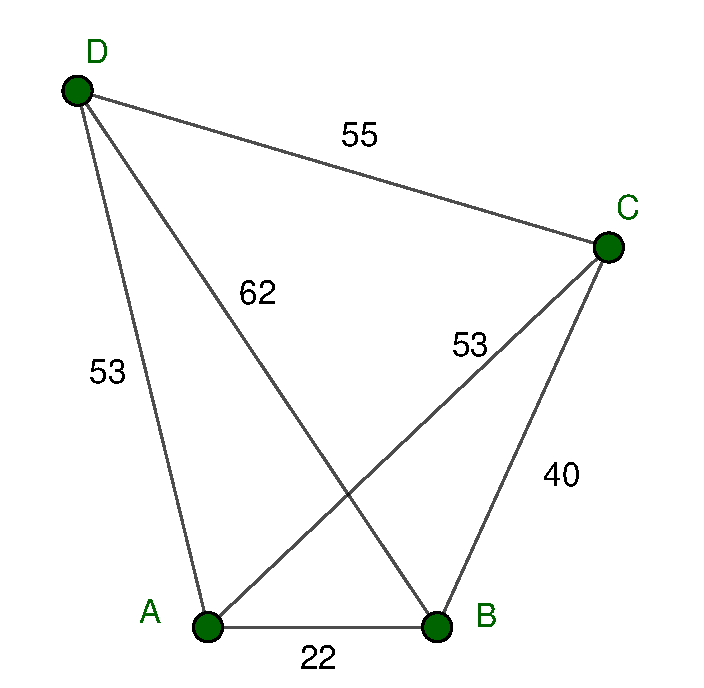
\includegraphics[width=.20\textwidth]{Distanze3.pdf}
%	\caption{\\Locations of \texttt{Neos4}.}
%	\label{fig:Neos4distance}
	%	\vspace{-10pt}
%\end{wrapfloat}
A permutation $\pi$ is the $4$-tuple of letters permuted so that $\pi_i$ is the location of facility $i$. For instance, $\pi_1 = \mathsf B$ means that we place facility $1$ into location $\mathsf{B}$.

We can imagine the situation graphically (Fig.~\ref{fig:Neos4instance}).


\begin{figure}%[htp]
	\centering
	\subfloat[\textit{Locations.}\label{fig:Neos4Locations}]{	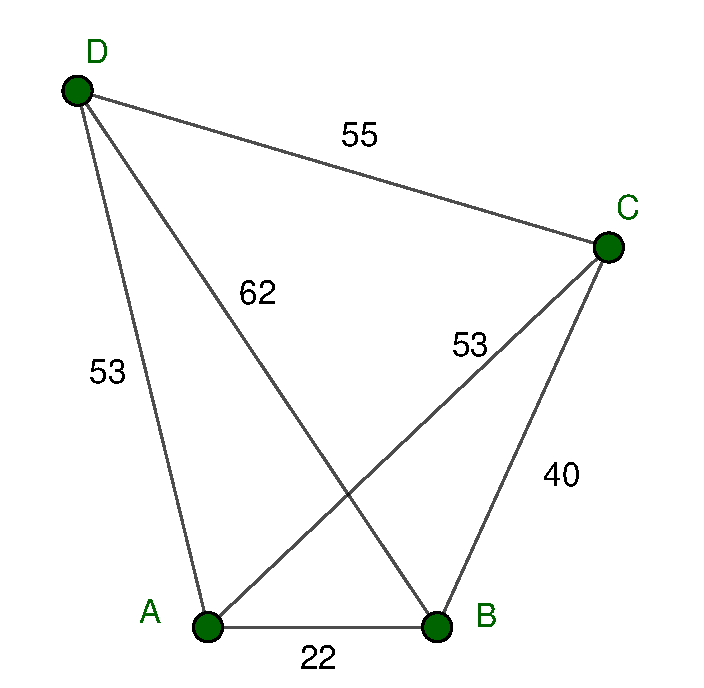
\includegraphics[width=.30\textwidth]{Distanze3.pdf}}\qquad
	\subfloat[\textit{Facilities.}\label{fig:Neos4Facilities}]{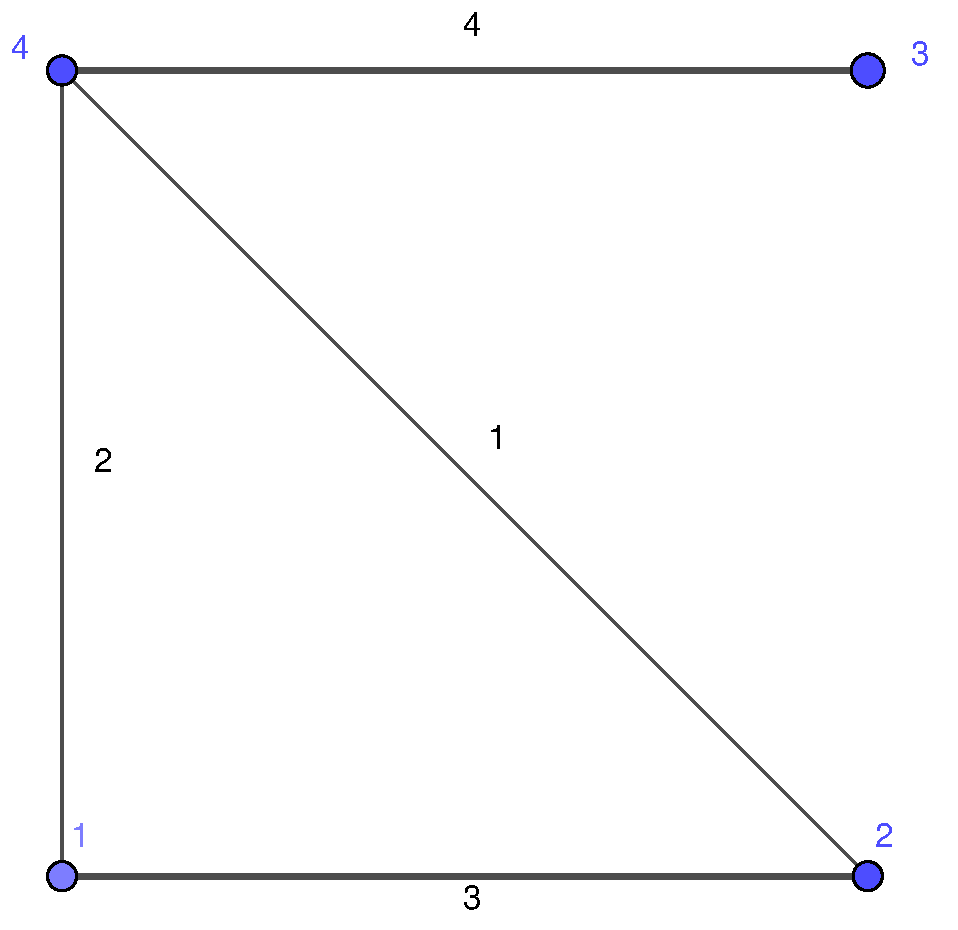
\includegraphics[width=.30\textwidth]{Flussi3.pdf}}
	\caption{Graphical description of \texttt{Neos4} instance.}
	\label{fig:Neos4instance}
\end{figure}

In figure~\ref{fig:Neos4Locations}  are shown locations of the \texttt{Neos4} instance. 

Locations (hence, the four point of the plane) are in\definecolor{verdescuro}{HTML}{006400} 
 \textcolor{verdescuro}{green}, while their distances are in black. Note that locations  $\mathsf A$ and  $\mathsf B$ are fairly close to each other. Instead, the other locations are far from each other, with similar distances. Our naive, basic intuition (but very useful for this section) suggest that facilities with the highest flow should be placed on locations  $\mathsf A$ and $\mathsf B$. 


On the other hand, figure~\ref{fig:Neos4Facilities} shows facilities of the same instance. Facilities are in \textcolor{blue}{blue}, while flows are in black. Thicker lines correspond to higher flows. If the flow is $0$, then no line is displayed. As we can see, facility $3$ is connected only with facility $4$, with a flow of $4$ (the highest one). If  Thus, our intuition proposes to place facility $3$ and $4$ close, while it is not necessary to place facilities $2$ and $4$ close to each other, since they only have a flow of $1$. 

In fact, the optimal solution of this instance  is $\pi=[\mathsf C,\mathsf D,\mathsf A,\mathsf B]$ with an objective function value of $z(\pi)=790$.
As we can see, facility $3$ is placed on location $\mathsf A$ and facility $4$ on location $\mathsf B$. This follows our previously intuition.

\subsubsection{Three basic algorithms}
So, how can one devise a greedy algorithm?
Remember that we want to minimize the quantity
\[
\sum_{i=1}^4\sum_{j=1}^4f_{ij}d_{\pi(i)\pi(j)}
\]

\noindent Since there must be a starting assignment, let us suppose that we are assigning location $\mathsf A$ to facility 1. Therefore, we set $\pi_1 = \mathsf A$. 

Now, how can we choose a second facility and a second location? 

%\bel{ 
Our first idea was to, at each step, minimize both flow and distance at the same time. This was a bad idea, since this choice is very good at the beginning, but later it has a severe impact on magnitude of last assignments.

Therefore, thinking about it, we have identified three different approaches:


\begin{description}
	\item[First approach] We start choosing facility with \textit{maximum} flow from $1$, this is~$2$. Now, the problem is to find the location to put facility $2$. We choose location that \textit{minimizes} the sum of distance from location already chosen. In this case, since we only chose $\mathsf{A}$, the location which minimizes the distance from $\mathsf{A}$, this is $\mathsf{B}$. Hence, we set $\pi_2=\mathsf{B}$.
	
	For the third assignment, we start choosing facility (not already taken) with highest flow from $2$, is $4$. For locations, we just evaluates the two sums: 
	$d_{\mathsf{A}\mathsf{C}}+d_{\mathsf{B}\mathsf{C}}=53 + 40 = 93 \quad \text{and} \quad	d_{\mathsf{A}\mathsf{D}}+d_{\mathsf{B}\mathsf{D}}= 53 + 62 = 115$.
	Since we want the minimum distance, we choose $\mathsf{C}$. Therefore, we just set $\pi_4=\mathsf{C}$. 
	
	The last possible assignment is $\pi_3=\mathsf{D}$. The final permutation built by this approach is $\pi=[\mathsf A, \mathsf B, \mathsf D, \mathsf C ]$ with objective function value $z(\pi)=864$.
	
	
	\item[Second approach] 
	This approach is fairly similar to the first one with the roles of facility and locations exchanged. So, we start choosing location with the \textit{minimal} distance $\mathsf{A}$, is $\mathsf{B}$. Now, we want to find facility which \textit{maximizes} the flow from already chosen facilities. This is simply facility $2$. Thus, we set $\pi_2=\mathsf{B}$. 
	
	For the third location we choose the closest one (not already taken) to $\mathsf{B}$, which is $\mathsf{C}$. Which facility comes now? Let us just do the math: $f_{13}+f_{23}=0+0=0$ and $f_{14}+f_{24}=2+1=3$. Since we want to maximize the flux, we set $\pi_4=\mathsf{C}$.
	
	The last one is forced, so $\pi_3=\mathsf{D}$. The final permutation is again $\pi=[\mathsf A, \mathsf B, \mathsf D, \mathsf C ]$ with objective function value $z(\pi)=864$.
	
	
	\item[Third approach] This approach is the simplest one. Choose the facilities with \textit{maximum} flow from facility 1 and assign it to the \textit{closest} location from \textcolor{verdescuro}{$\mathsf A$}. In this case, location \textcolor{verdescuro}{$\mathsf B$} is assigned to facility 2, therefore we set $\pi_2=\mathsf B$. 
	
	Now, $2$ has a positive flow only with facility 4, so we will chose that. As regards locations, $\mathsf C$ is the closest one to $\mathsf B$. Therefore, we set $\pi_4=\mathsf C$. 
	
	Last pair of facility/location is forced, hence $\pi_3=\mathsf D$. So, this approach builds again permutation $\pi=[\mathsf A, \mathsf B, \mathsf D, \mathsf C ]$ with objective function value $z(\pi)=864$.
\end{description}

We will transform these three approaches into three different algorithms, which will be named as \texttt{Greedy1}, \texttt{Greedy2}, \texttt{Greedy3}.

Some observations follows:
\begin{itemize}
	\item All these three methods are quite greedy. They tend to do the best at every step. The difference is that the third one is \virgolette{greedier} than the other two, since it considers only the current step, and not the past.
	\item We obtained three times the same final permutation. This is, in general, not true.
	\item \texttt{Greedy3} seems to be the fastest one, since no sum evaluation is necessary and it only looks for minimum/maximum in a vector.
	\item \texttt{Greedy3} is not an innovative strategy, this procedure is similar to the greedy algorithm for TSP proposed in~\cite{Kim2001}.
\end{itemize}





From now on, we return to the standard notations. Hence, facilities and locations will be denoted by numbers.

We are now going to describe the three algorithms in details.


Every greedy algorithm presented has three parameters on input: $q$, $n_1$, $n_2$ and two on output: $\bm p$ and $z_p$. 


\begin{description}
	\item[Input]The three parameters $q\in\{0,1\}$, $n_1,n_2\in\{1,\dots,n\}$ are used for the first assignment. They act as follows: \begin{itemize}
		\item If $q=1$, then algorithm assigns facility $n_1$ to location $n_2$. Hence, $ p(n_1)=n_2$.
		\item If $q=0$, then algorithm tries every possible initial assignment and chooses the best one. In this case, the algorithm does not use $n_1$ and $n_2$ and  can result in longer running time.
	\end{itemize}
	\item[Output] The final permutation is stored as $\bm p$ , a vector of $n$ components. 	$z_p$ represents the objective function value of $p$, i.e., $z_p = z(\bm p)$.

\end{description}

 %After the first assignment (thus after choosing $l_1$ and $f_1$),  matrices $\bm A$ and $\bm B$ are copied in two new matrices $\texttt{A}$ and \texttt{B}. 

Each of the three greedy algorithms creates two vectors $\bm v$ and $\bm l$, one for facilities and one for locations. 
These vectors represent the choice of the algorithm at each step. 

	Therefore, $v_i$ means that in step $i$ the algorithm choose the facility $v_i$ (and same thing for $l_i$). Thus at each step, after choosing $v_i$ and $l_{i}$, the algorithm add a new entry at the final vector $\bm p$, by setting $p_{v_i} = l_i$.



%\end{figure}

%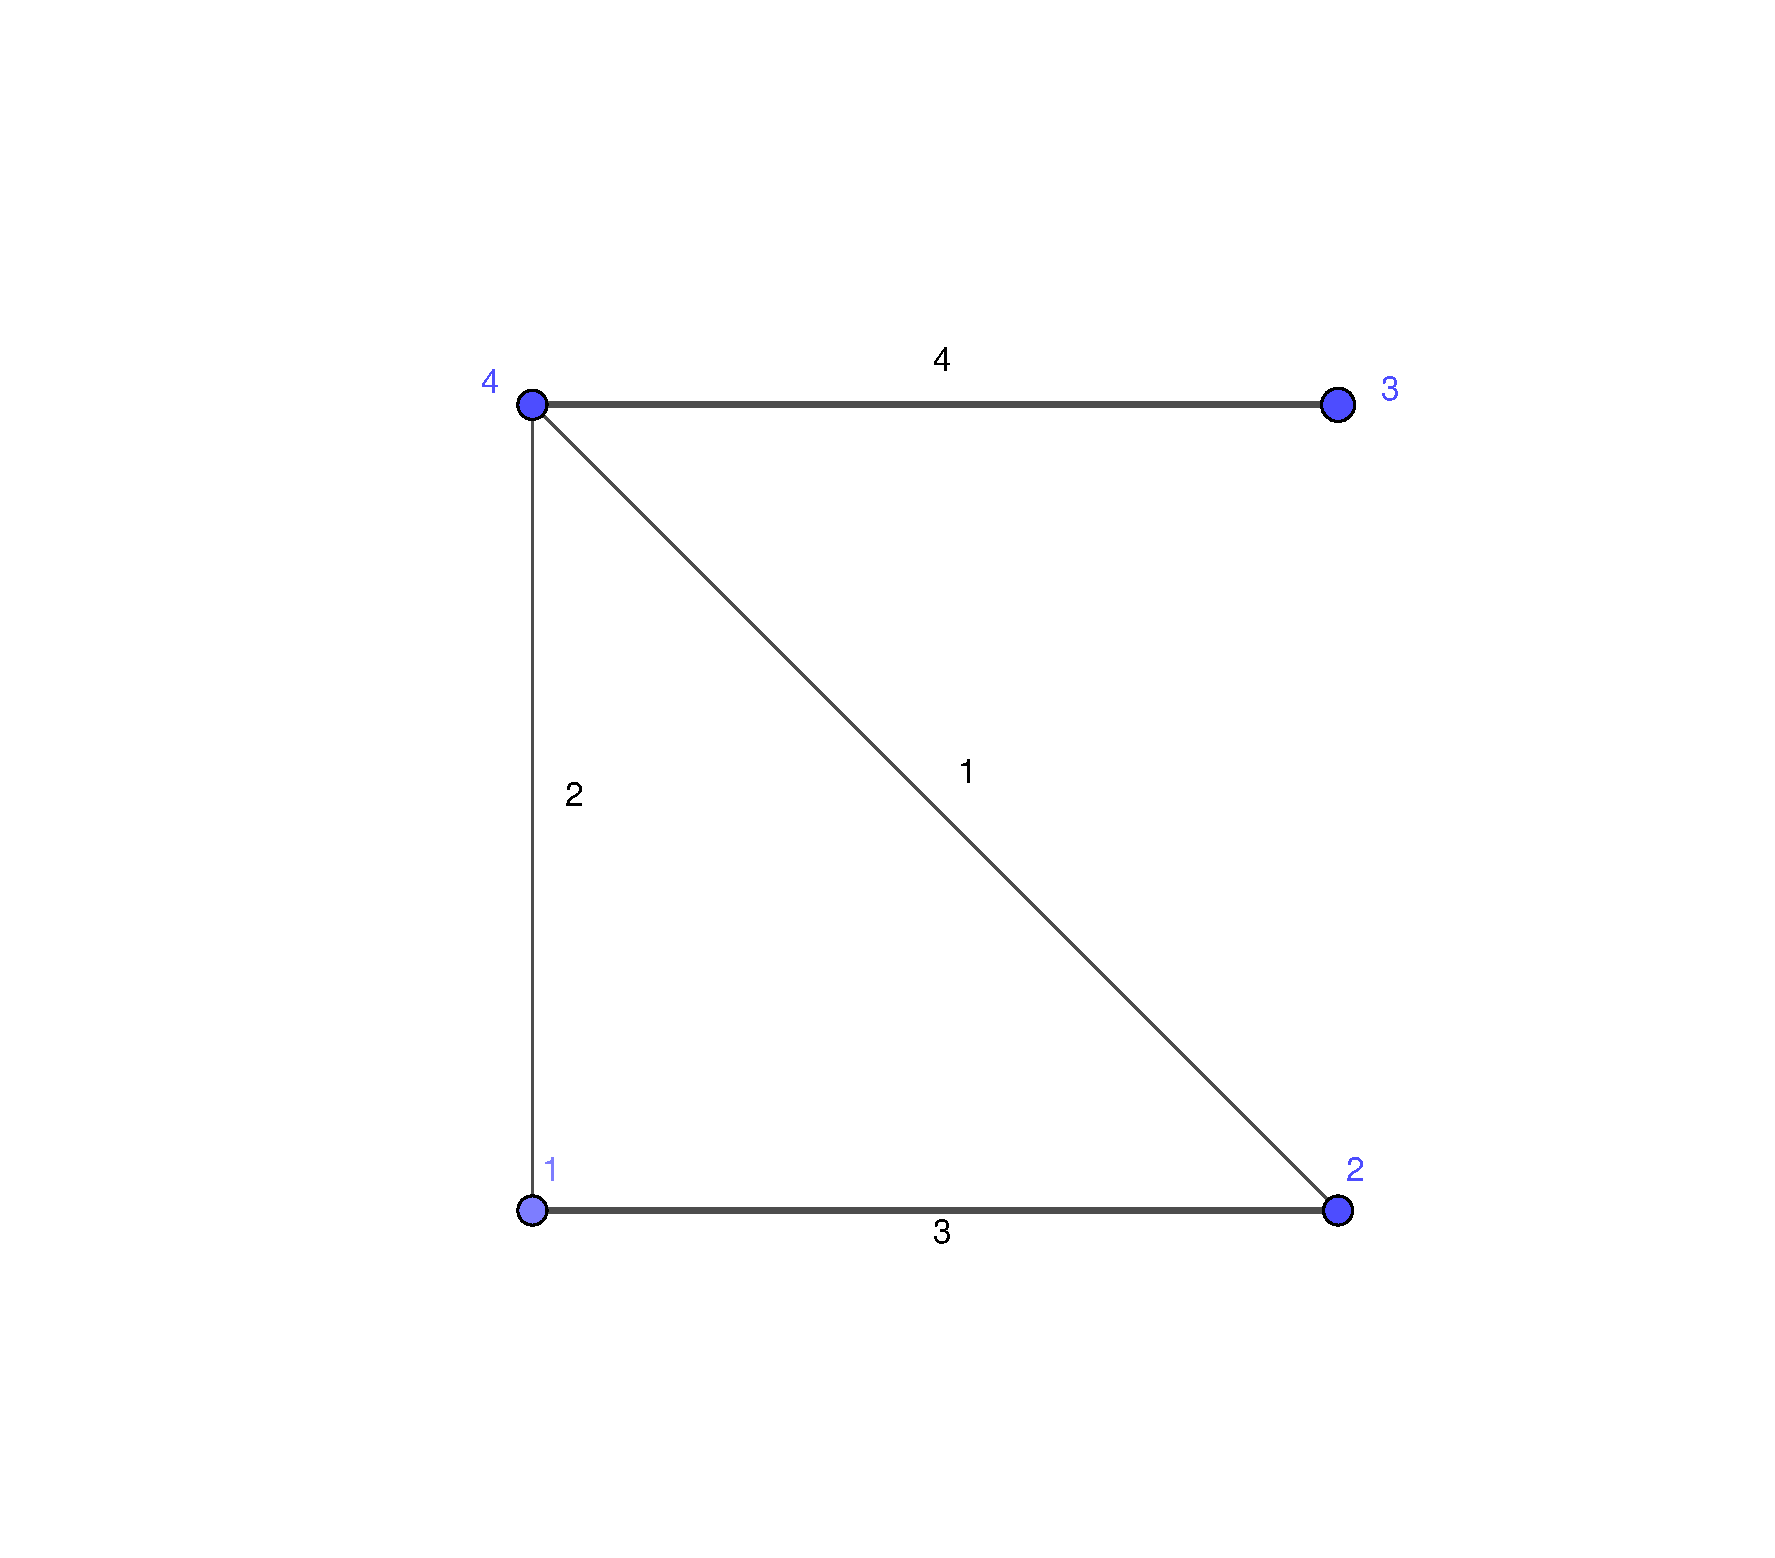
\includegraphics{flussi}

%after having assigned every facility to every location, these algorithms order  $\bm f$ using \texttt{ISORT}, a function of FTN95 which stores on the vector $\bm u_f$ the indices on the same order of the original vector $\bm f$. For example if $\bm f =[5,1,2,4,3]$, then $\bm u_f =[2,3,5,4,1]$. This allows to create the vector $\bm p$, by placing $p(i)=l(u_f)$ for every $i=1,\dots,n$.
%\dafinire

\subsection{\texttt{Greedy1}}


This algorithm represents the first approach we discussed in  section~\ref{sec:EsempioNeos4}. 

Pseudocode~\ref{Pseudocode: Gredy1} describes the algorithm in the symmetric case with $q=0$.




\begin{algorithm}%[htp]
	\KwIn{$n$,$\bm F$, $\bm D$,$n_1$, $n_2$}
	\KwOut{$p$, $z_p$}
	\tcc{initialisation}
	$v_1 \gets n_1$\; 
	$l_1 \gets n_2$\;
	$p_{v_1}\gets l_1$\;
	\tcc{main loop}
	\For{$i=1,\dots,n-1$}{
		Choose $v_{i+1}$, the facility with maximum flow from $f_{i}$\;
		Choose $l_{i+1}$, the location minimizing $\sum_{j=1}^if_{l_{i+1},j}\cdot d_{s,j}$\;
		$p_{v_{i+1}}\gets l_{i+1}$\;
	}
	Evaluate $z_p=z(p)$\;
	\caption[\texttt{Greedy1}]{\texttt{Greedy1} algorithm}
	\label{Pseudocode: Gredy1}
\end{algorithm}


As we said lines 1-3 represent the first assignment.

For the second assignment (and so on), \texttt{Greedy1}   chooses facility  $v_2$ which maximizes the flow from and to the previous ones (line 5); therefore 
\[
v_{i+1} = \argmax \Big\{\max\big\{f_{v_is}\big\},  \max\big\{f_{sv_i}\big\}\Big\}.
\]
 
\noindent After that,  the algorithm chooses location $l_{i+1}$, where facility $v_{i+1}$ will be placed. Location $l_{i+1}$ is chosen such that it minimizes the total flow sent to facilities already in place (line 6). In other words,
\begin{equation}
\begin{split}
l_{i+1} = \argmin\Biggl\{\displaystyle &\sum_{(k,j)\in \Omega} \left(f_{v_i k} d_{sj}+ f_{k v_i}d_{js}\right) \, \Big| \, s \in [n], s \neq l_1  \Biggr\}
\end{split}
\end{equation}


\noindent where $[n]=\{1,2,\dots,n\}$ and $\Omega$ is the set of pairs facility-location already assigned.

This procedure repeats for $i=1,\dots, n-1$ (line 4).

After choosing $v_{i+1}$ and $l_{i+1}$, \texttt{Greedy1} updates the final permutation setting $p_{v_{i+1}}=l_{i+1}$ (line 7).


In the case $q=0$, the algorithm starts again with every possible choice of $n_1$ and $n_2$. The best objective function value is stored.


We implemented \texttt{Greedy1} algorithm in Fortran language and  made it available on \href{https://github.com/Tommaso-Mannelli-Mazzoli/QAP/blob/master/Greedy1.f90}{GitHub}~\cite{Mazzoli2020}.


\subsection{\texttt{Greedy2}}
The second greedy algorithm follows the second approaches in~\ref{sec:EsempioNeos4}. Hence, it is similar to the first one, with the role of facilities and locations exchanged. 

Therefore, using the same notations as before, location $l_{i+1}$ is the closest one to $l_i$.

As regards facilities, $v_{i+1}$ is chosen as


\[
v_{i+1} = \argmin\Biggl\{\displaystyle \sum_{(k,j)\in \Omega} \left( f_{sk}\,d_{l_{i+1}j} +f_{ks}\,   d_{jl_{i+1}} \right)\,
\Big| \, s \in [n], s \neq v_k \, \forall k  \Biggr\}.
\]


\noindent The Fortran code we implemented for \texttt{Greedy2} can be found on \href{https://github.com/Tommaso-Mannelli-Mazzoli/QAP/blob/master/Greedy2.f90}{GitHub}.

\subsection{\texttt{Greedy3}}
The third greedy algorithm follows the third approach described in~\ref{sec:EsempioNeos4}.

For facilities, in each step, the algorithm consider the facility (not already chosen) with highest flow to the previous one.

For locations,  \texttt{Greedy3} considers the closest location (not already chosen) to the current one. 


In pseudo code~\ref{Pseudocode: Greedy3} it is shown the \texttt{Greedy3} algorithm for symmetric case. The Fortran code we implemented and used can be found on \href{https://github.com/Tommaso-Mannelli-Mazzoli/QAP/blob/master/Greedy3.f90}{GitHub}~\cite{Mazzoli2020}.

\begin{algorithm}%[htp]
	\caption{\texttt{Greedy3} algorithm}
	\label{Pseudocode: Greedy3}
	\KwIn{$n$,$\bm F$,$\bm D$,$n_1$, $n_2$}
	\KwOut{$p$, $z_p$}

\tcc{initialisation}
				$f_1 \gets n_1$\; 
				$l_1 \gets n_2$\;
				$p_{f_1}\gets l_1$\;
	\tcc{main loop}
			\For{$i=1,\dots,n-1$}{
	 				$v_{i+1}$ is the facility with maximum flow from $v_i$\;
					$l_{i+1}$ is the closest location to $l_i$\;
				$p_{v_{i+1}}\gets l_{i+1}$\;
			}
		Evaluates $z_p = z(\bm p)$.	
\end{algorithm}

\subsection{Implementation and Comparison}
We compared these three algorithms in order to choose which algorithm use to provide starting permutation for metaheuristic algorithms, that are described in the next chapter.



Table~\ref{tab:ConfrontiGreedy} shows percentage of deviation for various instance of \QAP. The case $q=0$ was chosen for every algorithm.  



\begin{table}
	\footnotesize
	\centering
		\caption[Comparison of Greedy algorithms.]{Comparison of Greedy algorithms. PD is the percentage deviation from the best known solution, $t$ is the running time in seconds.}
	\label{tab:ConfrontiGreedy}
	
	\begin{tabular}{l*{6}{S}}
		\toprule
		Instance& \multicolumn{2}{c}{\texttt{Greedy1}} &  \multicolumn{2}{c}{\texttt{Greedy2}} & \multicolumn{2}{c}{\texttt{Greedy3}} \\
		\cmidrule(lr){2-3}
		\cmidrule(lr){4-5}
		\cmidrule(lr){6-7}
&
{PD} & {$t$} &
{PD} & {$t$} &
{PD} &{ $t$}  \\
\midrule
 \texttt{lipa20a         }  &   3.18  &    0.0 &   5.89  &    0.0 &   3.10  &    0.0\\
\texttt{lipa20b         }  &   0.00  &    0.0 &  29.68  &    0.0 &   0.00  &    0.0\\
\texttt{lipa30a         }  &   2.78  &    0.1 &   4.17  &    0.1 &   2.62  &    0.0\\
\texttt{lipa30b         }  &   0.00  &    0.1 &  29.18  &    0.1 &  12.03  &    0.0\\
\texttt{lipa40a         }  &   2.11  &    0.5 &   3.49  &    0.5 &   2.03  &    0.0\\
\texttt{lipa40b         }  &  15.08  &    0.5 &  30.53  &    0.5 &  19.33  &    0.1\\
\texttt{lipa50a         }  &   1.74  &    1.4 &   3.12  &    1.3 &   1.72  &    0.1\\
\texttt{lipa50b         }  &  16.58  &    1.4 &  30.00  &    1.4 &  22.50  &    0.1\\
\texttt{lipa60a         }  &   1.58  &    3.3 &   2.74  &    3.2 &   1.60  &    0.2\\
\texttt{lipa60b         }  &  21.19  &    3.3 &  32.14  &    3.2 &  23.21  &    0.3\\
\texttt{lipa70a         }  &   1.45  &    6.9 &   2.49  &    6.8 &   1.37  &    0.5\\
\texttt{lipa70b         }  &  21.11  &    6.9 &  32.46  &    7.0 &  25.69  &    0.5\\
\texttt{lipa80a         }  &   1.28  &   13.2 &   2.25  &   12.9 &   1.22  &    0.8\\
\texttt{lipa80b         }  &  22.23  &   13.2 &  33.80  &   13.0 &  26.18  &    0.8\\
\texttt{lipa90a         }  &   1.17  &   23.5 &   1.99  &   22.3 &   1.12  &    1.3\\
   \texttt{lipa90b       }  &  23.31  &   23.1 &  33.51  &   22.6 &  25.23  &    1.2\\
\texttt{sko42           }  &   9.88  &    0.6 &  32.95  &    0.6 &  18.91  &    0.1\\
\texttt{sko49           }  &   8.22  &    1.3 &  31.46  &    1.2 &  16.40  &    0.1\\
   \texttt{sko56           }  &   8.44  &    2.4 &  31.14  &    2.4 &  17.52  &    0.1\\
\texttt{sko64           }  &   7.34  &    4.5 &  28.48  &    4.4 &  15.41  &    0.2\\
  \texttt{sko72           }  &   7.81  &    8.0 &  26.65  &    7.6 &  15.08  &    0.4\\
   \texttt{sko81         }  &   6.51  &   14.2 &  26.39  &   13.5 &  14.44  &    0.6\\
   \texttt{sko90           }  &   7.10  &   23.6 &  24.95  &   23.0 &  13.90  &    0.9\\
\texttt{sko100a         }  &   6.31  &   39.5 &  22.88  &   38.0 &  14.30  &    1.4\\
\texttt{sko100b         }  &   6.60  &   38.8 &  23.82  &   37.0 &  13.52  &    1.2\\
\texttt{sko100c        }  &   6.91  &   38.7 &  24.26  &   36.8 &  13.75  &    1.3\\
\texttt{sko100d        }  &   6.04  &   40.0 &  23.57  &   37.9 &  13.13  &    1.3\\
\texttt{sko100e        }  &   6.69  &   39.8 &  23.98  &   37.1 &  13.42  &    1.2\\
\texttt{sko100f         }  &   6.53  &   40.3 &  23.87  &   38.4 &  14.10  &    1.4\\
		\bottomrule
	\end{tabular}
\end{table}

We can see that all these greedy methods are not very precise, especially on instances \texttt{lipaxxb}. Nevertheless, as we stated at the beginning, they are commonly use only to built an initial guess for more advanced metaheuristic algorithms. 

Moreover, note that \texttt{Greedy3} is much faster than the other two (often with a difference of one order of magnitude), as a confirm of what we supposed. Thus, we will use it for metaheuristic methods presented in the next chapter, despite it shows larger PD values than \texttt{Greedy1}.